\documentclass[a4paper,11pt]{report}
\usepackage[utf8]{inputenc}
\usepackage[T1]{fontenc}
%\usepackage[utf8]{inputenc}
\usepackage{lmodern}
\usepackage{hyperref}

\usepackage[french]{babel}
%\usepackage{frnum}
\usepackage{numprint}
\usepackage{multirow}
\usepackage{graphicx}

\usepackage{csquotes}
\usepackage[]{glossaries}
\makeglossaries

\title{Nauteff P-1 Spécification}
\author{Emmanuel Gautier}

\usepackage[backend=biber]{biblatex}

\addbibresource{Nauteff-Biblio.bib}

\begin{document}
\maketitle

%%\newglossaryentry{MEMS}{name=Nom, description={}}

\newglossaryentry{babord} {
	name=bâbord,
	sort={BABORD},
	description={désigne le côté gauche d'un navire, en tournant le dos à la poupe}
}


\newglossaryentry{tribord} {
	name=tribord,
	description={le côté droit d'un navire, en tournant le dos à la poupe}
}

\newglossaryentry{cavalement} {
	name=cavalement,
	sort={CAVALEMENT},
	description={Mouvement le long de l'axe longitudinal du navire, c.à.d. d'avant en arrière, ce mouvement correspond à une accélération ou un ralentissement.}
}

\newglossaryentry{embardee} {
	name=embardée,
	sort={EMBARDEE},
	description={Mouvement latéral du navire, c.à.d. vers son côté. Il est souvent provoqué par les rafales de vent et la houle. Il est souvent liée à la gîte et à la dérive}
}

\newglossaryentry{I2C} {
	name=I2C,
	description={Inter-Integrated Circuit en englais. C'est un bus de communication série à 2 fils à courte distance.}
}

\newglossaryentry{gite} {
	name=gîte,
        sort=gite,
	description={inclinaison latérale d'un navire. La gîte est généralement due au vent.}
}

\newglossaryentry{MEMS} {
    name=MEMS,
    sort=MEMS,
    description={Micro Electro Mechanicals Systems ou, en français, systèmes micro électromécaniques. Parmi ces systèmes figurent le magnétomètre, l'accéléromètre et le gyromètre.}
    }

\newglossaryentry{compas} {
    name=compas,
    sort=COMPAS,
    description={instrument de navigation indiquant le nord magnétique}
}

\newglossaryentry{NMEA}
{
	name={NMEA}, % le terme à référencer (l'entrée qui apparaitra dans le glossaire)
	description={National Marine Electronics Association. Cet organisme américain a créé les protocoles NMEA~0183 et NMEA~2000}, % la description du terme(sans retour à la ligne)
	sort={NMEA}, % si le mot contient des caractère spéciaux, ils ne seront pas pris en compte
	plural={NMEA} % la forme plurielle du terme
}

\newglossaryentry{NMEA0183}
{
	name={NMEA0183}, % le terme à référencer (l'entrée qui apparaitra dans le glossaire)
	description={Protocole Normalisé et non officiellement documenté défini par la NMEA utilisé par des appareils de navigation}, % la description du terme(sans retour à la ligne)
	sort={NMEA0183}, % si le mot contient des caractère spéciaux, ils ne seront pas pris en compte
	plural={NMEA0183} % la forme plurielle du terme
}

\newglossaryentry{pilonnement} {
    name=pilonnement,
    sort={PILONNEMENT},
    description={Mouvement vertical du navire, c.à.d. de bas en haut et de haut en bas. ce mouvement est généralement provoqué par les vagues.}
    }

\newglossaryentry{roulis} {
	name=roulis,
	description={ Mouvement d'oscillation d'un bateau autour de l'axe longitudinal (en général sous l'effet de la houle ou du vent)}
}

\newglossaryentry{quaternion} {
	name=quaternion,
	sort={QUATERNION},
	description={Nombre hypercomplexe formé par une partie réelle et 3 parties imaginaires, il servent à représenter l'orientation du navire}
}

\newglossaryentry{lacet} {
	name=lacet,
	description={mouvement de rotation par rapport à l'axe vertical du navire}
    }

\newglossaryentry{tangage} {
	name=Tangage,
	description={mouvement de rotation par rapport à l'axe transversal du navire}
    }

\newglossaryentry{UART} {
	name=UART,
	description={Universal Asynchronous Receiver Transmitter soit émetteur-récepteur asynchrone universel, aussi appelée liaison série.}
}


\begin{abstract}
Ce document contient la spécification du prototype Nauteff P-1.
\end{abstract}

\tableofcontents
\listoftables
\listoffigures


\chapter{Buts du document}
\section{Buts}
Ce document décrit la spécification du Nauteff P1. Il sert de référence
pour tous les acteurs du projet.
Il contient les exigences techniques du Nauteff,
la description de son comportement et de ses fonctions. 

\section{Guide de lecture}
C'est le document de référence principal décrivant
les exigences techniques et opérationnelles et la description
des fonctions du système. Il est destiné à tous les acteurs
participant à la définition du système ou à sa réalisation.

Bien que décrivant le système il n'est pas un manuel d'utilisation.

Le détail des fonctions de calculs et algorithmes est contenu
dans un autre document à venir.

\chapter{Documents applicables et de référence}

Ce document sert de référence pour le développement.

\printbibliography[heading=none]

\chapter{Glossaire}

%\printglossary[title={}, toctitle={}]
\printglossary

\chapter{Présentation du Pilote automatique}
\section{Objectifs}
Nauteff P-1 est une maquette de pilote automatique pour navires à voile ou à moteur d'une taille comprise entre 5m et 24m.
Cette maquette sert à évaluer et mettre au point le pilote automatique et améliorer son logiciel.

L'objectif d'un Pilote automatique sur un bateau 
est d'agir sur sa barre afin de maintenir le cap d'un navire.
Il doit aussi traiter des informations sur les conditions
de navigation et le fournir à d'autres appareils.
Il utilise les informations de ses capteurs, et lorsqu'elles
sont disponibles celles d'autres appareils.


\section{Environnement du système}

\begin{figure}
	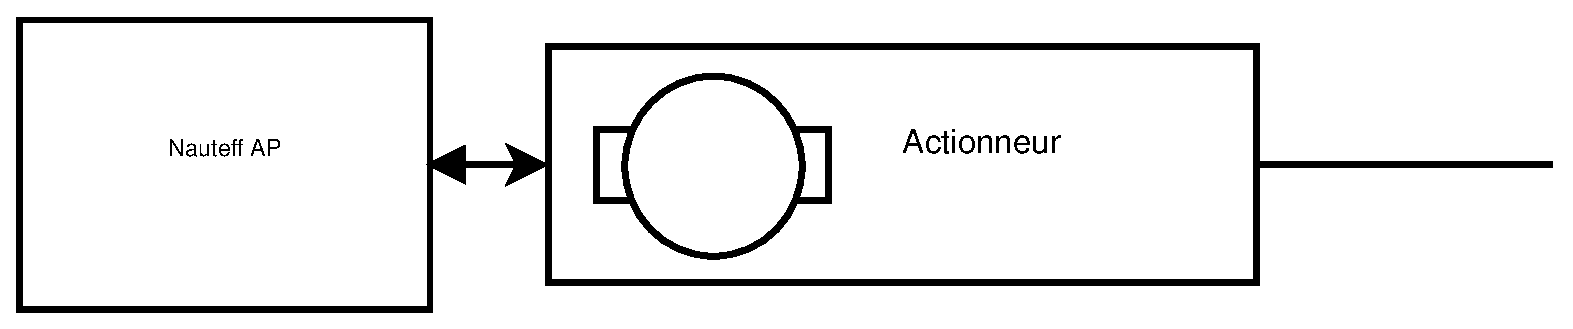
\includegraphics[width=8cm, keepaspectratio]{Nauteff-AP-Environment.eps}
	\caption{diagramme général}
\end{figure}

L'environnement du Nauteff~P-1 comprend:
\begin{itemize}
	\item un ordinateur avec les outils de développement et la sonde;
	\item un alimentation 12V;
	\item un vérin électrique;
	\item des instruments de navigation: GPS, loch, gyrouette,\dots
	\item un ou plusieurs équipiers du navire;
	\item un utilisateur.
\end{itemize}

Nauteff P-1 est principalement utilisé et stocké dans un bureau
au chaud et au sec. Lors des essais il est à l'intérieur d'un navire
et modérément protégé de l'humidité.

Il est relié à un ordinateur par l'intermédiaire d'un sonde qui
alimente la calculateur et qui permet de charger le logiciel
de contrôler l'exécution et de faire le débogage.

Au bureau l'ordinateur est de type station de travail et l'alimentation
de l'actionneur est fourni par une alimentation stabilisée.
Lors des essais à bord d'un navire le l'ordinateur est un petit modèle
portable, et économe en courant; l'ensemble est alors alimenté par
la batterie de servitudes du navire.

L'équipage confie la commande de la barre au Nauteff pour réaliser d'autres
tâches ou pour se reposer. Il attend un bon suivi de cap, exige d'être
alerté en cas de changements de conditions ou si
le Nauteff ne peut plus remplir sa fonction.


\subsection{Interfaces du système}


\subsection{Utilisateurs}
Les utilisateurs sont les concepteurs du système ou des navigateurs prenant part à son développement.
Le prototype n'est pas destiné aux utilisateurs.

\subsection{Environnement en contexte opérationnel}

\subsection{Environnement de développement et de mise au point}

\section{Conventions d'orientation et d'unités\ldots}
Nauteff utilise les unités courantes des marins en externe.
Par contre, en interne il utilise les unités du système MKS, les radians
pour simplifier le codage et éviter les erreurs de conversion.
Le choix des directions des axes x, y et z du repère du navire
sont : x vers l'avant, y vers bâbord (à droite) et z vers le bas.
Cette orientation des axes est couramment utilisée
par la marine et l'aviation.
Elle est appelée convention NED pour North, East Down.
Elle permet d'avoir un repère direct.

\begin{figure}
	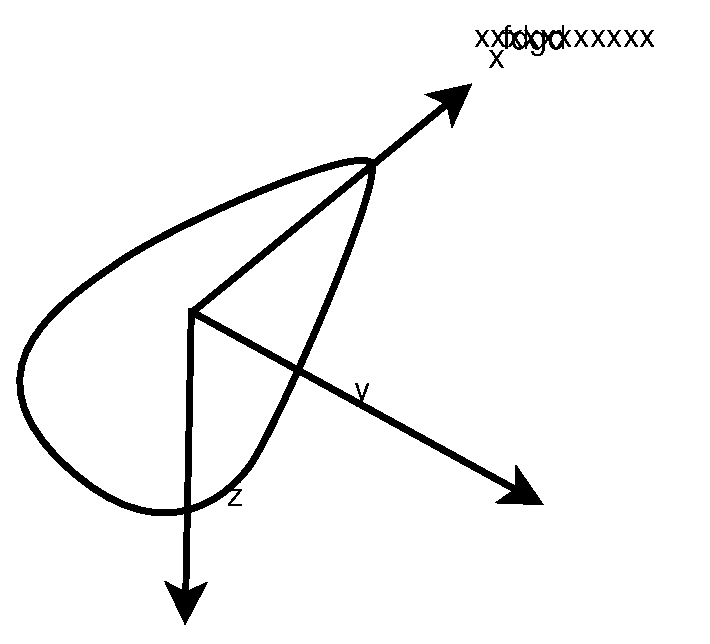
\includegraphics[height=5cm]{orientation.eps}
	\caption{Convention d'orientation}
\end{figure}


\chapter{Spécification générales}
\section{Description des services attendus}

\section{Description des générale du matériel}

Nauteff 


\section{Description des générale des fonctions}
\section{Exigences opérationnelles}
\subsection{Contraintes d'exploitation}
\subsection{Modes de fonctionnement}
Nauteff comporte un mode veille, un mode Automatique et un mode paramétrage.
\subsection{Transition entre modes}
\subsection{Exigences de l'environnement}
Nauteff P-1 est conçu pour supporter une ambiance saline avec une humidité
saturante permanente et un température de fonctionnement comprise entre   0\degres C et +30\degres C.
Nauteff doit aussi supporter des vibrations.
La tension d'alimentation du Nauteff doit être comprise entre 10V et 20V, il consomme moins de 50~mA en fonctionnement, hors moteur.
Il permet de commander un actionneur avec une charge inductive consommant jusqu'à
12\ A en régime permanent.
Nauteff est protégé contre les surcharges et court-circuits de l'actionneur et 
contre les inversions de polarité de l'alimentation.
\subsection{Capacité}
\subsection{Performances}
\begin{table}
\begin{tabular}{|c|c|}
	\hline 
	Temps de démarrage &  < 2s \\ 
	\hline 
	Entrée NMEA& décodage de trames transmises à \numprint{230400} bps \\ 
	\hline 
	Réaction à une embardée & 1s max \\ 
	\hline 
	&  \\ 
	\hline 
	&  \\ 
	\hline 
\end{tabular}
\caption{Performances}
\end{table}


\subsection{Paramétrage}
Le Nauteff P-1 comporte des paramètres suivants:
\begin{itemize}
	\item caractéristiques du moteur: courants en butée et à vide, inertie;
	\item valeurs d'étalonnage des capteurs;
	\item vitesse de réaction;
	\item amplitude de réaction;
	\item compensation d'\gls{embardee};
	\item angle de virement de bord et amplitude du mouvement de l'actionneur;
	\item valeurs limites;
	\item coefficients de pilote à définir;
	\item \ldots
\end{itemize}
Dans la version d'évaluation ces paramètres sont dans des constantes
("codées en dur") modifiées avec les outils de développement.

\subsection{Contraintes entre le matériel et le logiciel}
\subsection{Sûreté de fonctionnement}

\subsection{Exigence organisationnelles}

\subsection{Exigences de mise au point et de maintenance}
Nauteff P-1 est un prototype monté sur carte d'essai et permet un
accès facile à tous les signaux et des modifications rapides et aisées.

\section{Exigences techniques}



\section{Interface homme machine}
Nauteff est équipé d'un clavier à 6 touches fugitives (contact NO).

\begin{table}
\begin{tabular}{|c|c|c|c|}
	\hline 
	Libellé    & couleur & fonction principale &  \\ 
	\hline 
	``Auto''   & noire & Mise en mode automatique &  \\ 
	\hline 
	``Veille'' & noire & Mise en veille &  \\ 
	\hline 
	``+1''     & verte & Changement de cap 1\degres~vers tribord &  \\ 
	\hline 
	``-1''     & rouge & Changement de cap 1\degres~vers bâbord  &  \\ 
	\hline 
	``+10''    & verte & Changement de cap 10\degres~vers tribord &  \\ 
	\hline 
	``-10''    & rouge & Changement de cap 10\degres~vers bâbord  &  \\ 
	\hline
\end{tabular} 
\caption{Touches du clavier}
\end{table}
Il y en a 6 en tout.

\chapter{Description générale du matériel}

\section{Raccordements}

\begin{tabular}{|c|c|p{6cm}|}
	\hline
	type & Nbre & description \\
	\hline
    Alimentation & 1  & 10 à 18 V, 2A, 32A max  \\
    \hline
	UART & 3 & RS232
	           \newline \numprint{4800} à \numprint{38400} bits/s
	           \newline Interface avec les instruments
	           \\
	\hline
	UART & 1 &  niveau 3.3V ou TTL
                \newline \numprint{230400} bits/s
                \newline sortie vers sonde et PC de dév.\\
	\hline
	I2C & 1 & 3.3V ou TTL \numprint{100} et \numprint{400}kbits/s
	          \newline Pour raccordement utlérieurs\\
	\hline
	SPI & 1 &  Maître, MISO, MOSI, CLK et 2 CS
	           \newline à partager avec capteurs MEMs\\
	\hline
    CAN & 1 & Pour raccordement futur au bus NMEA 2000 \\
	\hline
	Moteur & 1 & Pour moteur à courant continu 
	             \newline 2 fils, 10A continu, 30A max\\
	\hline
	Clavier & 1 & 6 fils pour les contacts des touches
	              \newline quelques fils pour LED, à définir \\
	\hline
	alarme & 1 &  Contact avec Vcc \\
	\hline
\end{tabular}

\subsubsection{Alimentation électrique}
Nauteff fonctionne avec une alimentation électrique
très basse tension nominale de 12V et l'alimentation de la sonde.
l'alimentation 12V répond aux exigences de la section exigences de l'environnement.

\subsection{protocoles de communications}
Le document \cite{NMEARevealed} décrit le protocole de communication.

\subsubsection{Clavier}
Nauteff comporte un clavier à 6 touches fugitives (aussi appelées à contacts NO).

\subsubsection{Bus de communication UART, \ldots}
Nauteff comporte une interface série RS-232 principalement utilisée
pour la communication avec un ordinateur pour le développement et
la mise au point.

La norme \gls{NMEA} prévoit un bus RS-422, cependant cette interface
permet des échanges d'information avec des appareils utilisant
ce protocole et peu exigeants.
C'est l'\gls{UART} qui est utilisée pour la communication avec le PC.

\subsubsection{Capteurs MEMS}
Nauteff P-1 comporte les capteurs \gls{MEMS} suivants :
\begin{enumerate}
	\item un magnétomètre (LSM6DS33);
	\item un gyromètre (LPS25H);
	\item un accéléromètre(LPS25H);
	\item un capteur de pression atmosphérique (LIS3MDL);
	\item des capteurs de température.
\end{enumerate}
Ces capteurs sont dans les circuits intégrés de ST Microelectronics et montés
sur une carte d'évaluation Pololu AltIMU-10 v5. La communication entre ces capteurs et le STM32 utilise un bus \gls{I2C}. Les capteurs de température et de pression atmosphérique nz sonrt pas utilisés.

\subsubsection{Commande du moteur}
Nauteff comporte une unité de commande et de contrôle du moteur de l'actionneur.
Cette unité permet de commander la marche du moteur de l'actionneur
dans les deux sens et de mesurer l'effort du moteur (couple),
de détecter la butée, un courant excessif ou un court-circuit et un courant nul
ou anormalement faible et de surveiller la tension d'alimentation.
La commande du moteur comprend aussi une estimation de la position du moteur.

\subsubsection{Alarme sonore}
L'alarme sonore appelle l'attention du navigateur que le Nauteff ne peut plus
assurer ses fonctions ou que des valeurs sont en dehors des limites fixées
et que la navigateur doit intervenir.

\subsubsection{Écran}
Dans la version d'évaluation Nauteff P-1 n'a pas d'écran et sort les information
sur USART2 pour un affichage sur l'écran de l'ordinateur de développement.
Ça serait dommage de se priver d'un écran, il en faudra au moins un petit avec quelques caractères.

\subsubsection{Voyants}
Nauteff P-1 comporte les voyants suivant :
\begin{itemize}
	\item Voyants de mise sous tension;
	\item Voyant vert indiquant l'enclenchement du pilote;
	\item Voyant rouge lors d'un mouvement vers tribord de l'actionneur;
	\item Voyant vert lors d'un mouvement vers tribord de l'actionneur;
	\item Voyant indiquant le fonctionnement de l'USART;
	\item Selon les besoins de mise au point.
\end{itemize}
Rappel : Le rouge indique le côté bâbord (gauche) et le vert indique le côté tribord.

\section{microcontrôleur}
Le microcontrôleur est un STM32L476RE monté sur carte Nucleo
qui comprend la sonde, et une interface UART et est relié
à un PC de développement par liaison USB.

\section{Alimentation}

\section{Commande et contrôle de l'embrayage et du moteur}

\section{Capteurs d'orientation}

\section{entrées et sorties}

\subsection{UART2}
UART2 sert aux communications avec le PC de développement.
Elle utilise un débit élevé et sert à échanger les informations
entre le pilote et une interface et à envoyer des informations
de mise au point.

\subsection{UART1, UART3}
Ce sont des liaisons série RS232 avec un débit de 4800 bits/s,
8 bits et un bit de stop. Elles utilisent le protocole NMEA0183
décrit dans \cite[NMEA révélé][]{NMEARevealed}.
Leur débit peut être porté à \numprint{9600} ou \numprint{38400} bits/s.

\section{SPI1}


\chapter{Description détaillée du logiciel}

\section{Étalonnages}

\subsection{Capteurs MEMs}

\subsection{Commande de barre}
La commande de position barre est obtenue avec ~\eqref{eq:calculPID}.
C'est un calcul de régulation PID.

\begin{equation}
	\label{eq:calculPID}
	Cmd = K_p * Ecart + K_d * Gyr + K_i * Cumul
\end{equation}

\section{Lecture du clavier}

\begin{tabular}{|c|p{6cm} |}
	\hline
	 Touche & Action  \\ \hline
	\multicolumn{2}{|c|}{En mode veille} \\ \hline
	 Appui sur ``Auto'' & Passage en mode suivi de cap\\ \hline
	 Appui sur Veille & Sans effet \\ \hline
	 Appui +1 &  Mise en marche de l'actionneur vers tribord \\ \hline
	 Appui -1 &  Mise en marche de l'actionneur vers bâbord \\ \hline
	 +10 & Sans effet     \\ \hline
	 -10 &  Sans effet    \\ \hline
	\multicolumn{2}{|c|}{En mode auto} \\ \hline
	%pression sur touche ``Auto'' & changement de mode : suivi de cap, %suivi de vent et suivi GPS     \\ \hline
	Pression sur ``Veille'' & Mise en mode veille     \\ \hline
	+1, -1, +10, -10 & modification de la consigne de cap     \\ \hline
	+1, +10 simultanément &  incrément de la consigne de 90\degres    \\
	-1, -10 simultanément &  décrément de la consigne de 90\degres    \\ 
	 \hline
\end{tabular} 
\\

La consigne est toujours arrondie au degré
et est toujours comprise entre 0 et 359\degres.
\\

L'appui sur la touche ``Auto'' met le Nauteff en mode automatique de suivi de cap.
La touche ``Veille'' met le Nauteff en mode veille.
En mode veille l'enfoncement des touches ``+1'' et ``-1'' commandent le déplacement du vérin vers tribord et bâbord.
En mode automatique, un appui sur les touches ``+1'' et ``-1'' ``+10'' et ``-10''
changent le cap de 1\degres~ ou 10\degres~ vers tribord ou bâbord.
Le maintient enfoncé des touches ``+1'' et ``-1''

\subsection{Veille}

\subsection{Maintient du cap}

\subsection{Configuration et réglages}

\section{Détermination de l'orientation du navire}
\subsection{Lecture des valeurs des capteurs}
Lors de l'initialisation Nauteff configure les capteurs :
Nauteff utilise l'accéléromètre, le gyromètre et le magnétomètre.
Il lit ces valeurs à chaque fois qu'elle sont disponibles,
les accumule et les compte.

\subsection{Calculs d'orientation}
À une cadence de 10Hz, Nauteff calcule la moyenne des valeurs,
applique les corrections issues de l'étalonnage et
calcule les nouvelles valeurs d'orientation.
Nauteff envoie ces valeurs sur la sortie UART2.


\section{Décodage des informations en entrée}

\section{Maintien du cap}


\section{Commande et surveillance du moteur}
Nauteff contrôle l'embrayage, le moteur et la tension d'alimentation.
Il assure les fonctions suivantes:
\begin{itemize}
	\item Envoi de la commande d'embrayage;
	\item Mise en marche et arrêt du moteur;
	\item Surveillance de la tension d'alimentation;
    \item Mesure du courant du moteur;
	\item Estimation de la position de la barre;
	\item Envoi d'alarme de détection de butée de moteur bloqué ou de court-circuit;
	\item Envoi d'information sur l'effort du moteur (dureté de la barre) et de la position aux autres tâches.
\end{itemize}

Le contrôle du moteur comprend les commandes suivantes:
\begin{itemize}
	\item Embrayage ;
	\item débrayage ;
	\item demande de la position de la barre ;
	\item déplacement de la barre à bâbord ou tribord pendant un temps donné
	\item déplacement de la barre à un angle donné;
\end{itemize}

L'angle de barre est estimé. Il est en général limité à environ 15\degres{}, cet angle dépend du montage du vérin ou de la barre du bateau.

La tension d'alimentation et le courant du moteur sont mesurés à une cadence de 100Hz quand le moteur tourne. Lorsque le moteur tourne 
\begin{figure}
	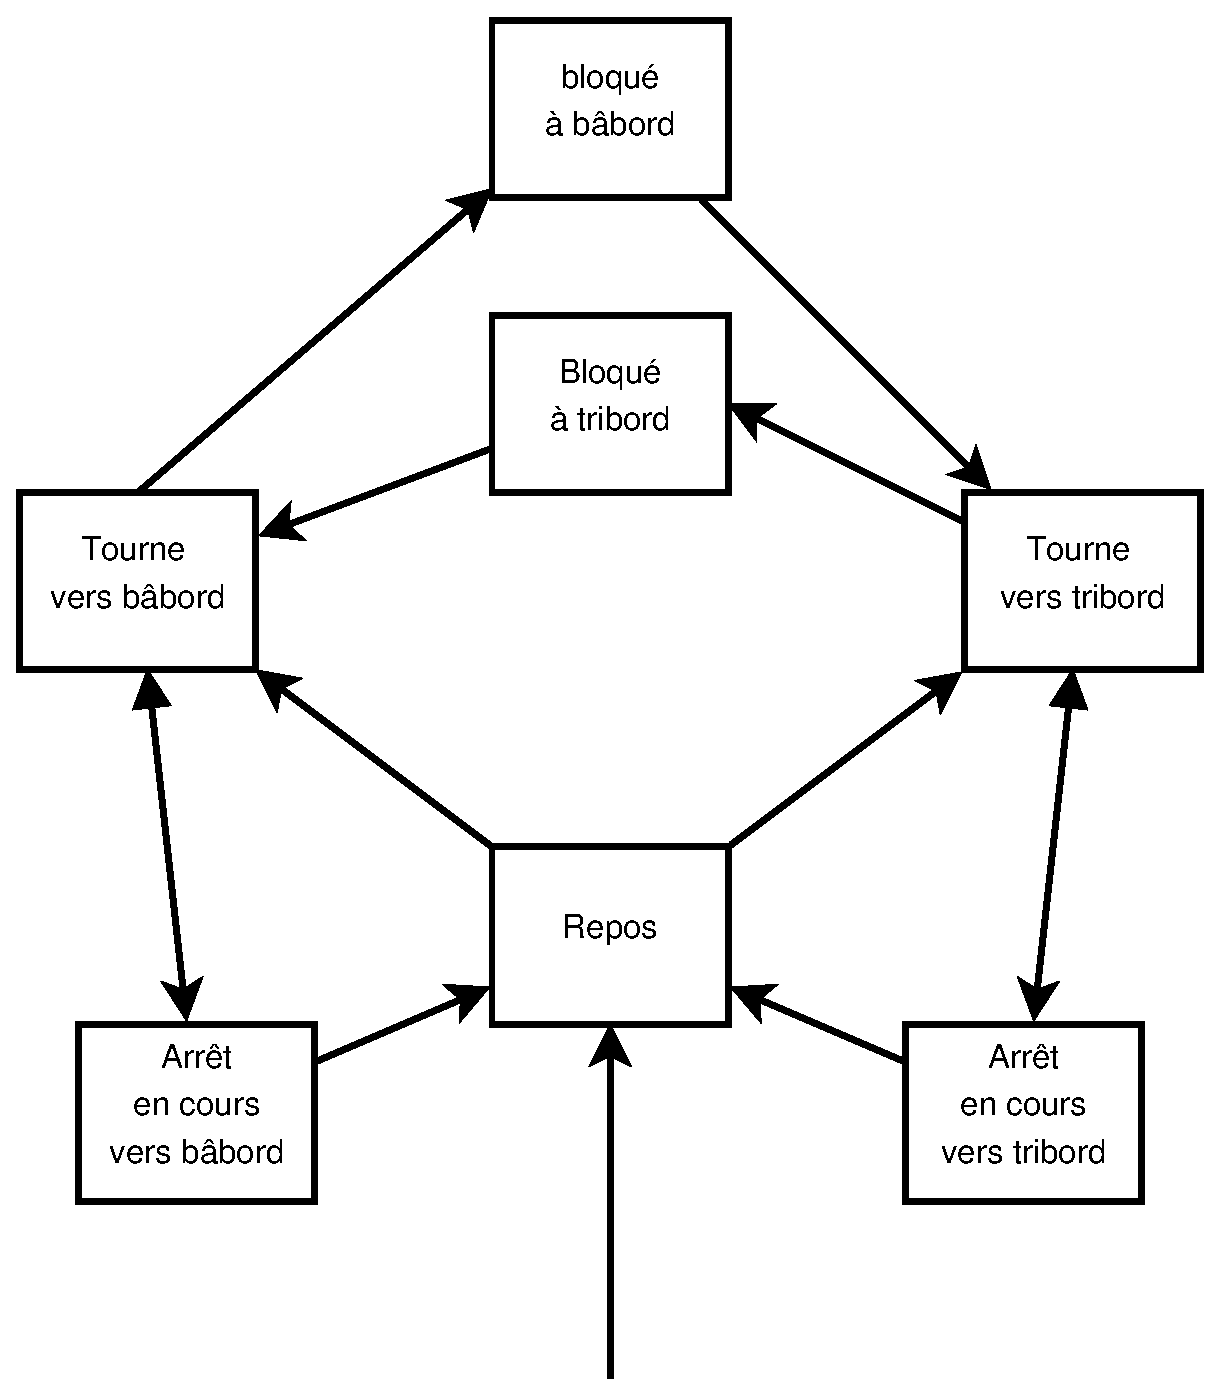
\includegraphics[height=5cm]{MotorStatus.eps}
	\caption{États du moteur}
\end{figure}


\section{Émission d'alarmes}

\begin{itemize}
	\item Moteur bloqué;
	\item Moteur en court-circuit;
	\item Écart de cap au delà de la limite (à définir);
	\item Tension d'alimentation hors limites;
	\item Mode panique déclenché.
\end{itemize}

\section{Panique}
En cas de défaut du logiciel ("plantage") lors du fonctionnement, Nauteff doit envoyer une commande de bas niveau pour arrêter le moteur
et déclencher l'alarme.

 
\section{Envoi d'informations}
\subsection{Informations de mise au point}
\subsection{Informations pour une interface du Nauteff}

\chapter{Interfaces}
\section{Interface NMEA-0183}
Nauteff peut recevoir et émettre des données au format NMEA-0183.
Ce protocole utilise des liaisons RS422 à \numprint{4800} bits/s 8N1 parfois 7N2.
Lorsque plusieurs appareils sont reliés, un seul peut parler. 
La vitesse est portée à des valeurs plus élevées par certains appareils.
Les données sont dans des "phrases" d'un logueur limitée à 82 caractères
avec une somme de contrôle et une séquence <CR><LF>.
Les phrases reconnues par Nauteff commencent
par un \$, deux lettres majuscules indiquant la provenance
et trois lettres majuscules indiquant le type de phrase.
\\

Nauteff comprend les types phrases suivants :

\begin{itemize}

	\item[RMC]  Recommended Minimum Specific GNSS. 
	contient  la position (latitude et longitude),
	la vitesse par rapport au sol (Speed Over Ground),
	le cap suivi (Course Over Ground),
	l’heure et la date. C’est une des phrases les plus utilisées des récepteurs GPS;

    \item[GGA]: Global Positioning System Fix Data. 
    Contient la position GPS, la qualité de la mesure,
    le nombre de satellites utilisés,
    l'altitude, etc;

    \item [GLL]: Geographic Position - Latitude et Longitude,
    Contient la latitude, la longitude** et l'heure du fix;

    \item [VTG] - *Track Made Good and Ground Speed. 
    Contient le cap par rapport au nord vrai ou magnétique
    et la vitesse sur le fond (ground speed) à partir du GPS;

    \item[VHW] : Water Speed and Heading***
     Donne **la vitesse du bateau par rapport à l’eau (speed through water) et
     le cap du bateau. C’est la phrase standard pour mesurer la vitesse dans l’eau (souvent émise par un loch/sonde);

    \item[VBW] :Dual Ground/Water Speed
    Contient à la fois vitesse par rapport à l’eau et
    la vitesse sur le fond avec leurs statuts de validité;

    \item[MWV] : Wind Speed and Angle.
     Contient la vitesse du vent et l’angle du vent (souvent par rapport à l’axe du bateau).
     C’est une des phrases les plus communes pour une girouette/anémomètre.

\end{itemize}

\section{Interface Nauteff}


turn port|starboard <NNN>
mode idle|headind [<NNN>]


\end{document}
